\mySection{System Overview}
Our system's primary goal is to help school faculties perform roll calls with ease.
Traditional roll calls require teachers to call the names of students individually to record students' attendance,
while PyRollCall let a teacher simply take a photo of the entire class and record students' attendance
using Facial Recognition, thus saving more time for both teachers and students in classes.
\vspace{0.5cm}

Before we can actually use the system to recognize the faces of students, teachers should
collect at least 10 to 15 photos for each student, and let the system compute the measurement (or embedding) of each face.
These pre-computed facial embeddings will be saved in the database for later use.
When a face is caputured in roll calls, the system will use k-NN classification and votes
to determine whom the face belongs to.
\vspace{0.5cm}

Users (typically teachers) should also enter the names of the courses they teach into the system.
For each course, enter which students are taking it including students' names and IDs.
PyRollCall's GUI is demonstrated in figure~\ref{fig:systemAppearance}. 
After setting up these data into the system, PyRollCall will be ready to perform roll call for a specific course
using facial recognition. To summarize, users should (1) collect around 10 to 15 photos for each student and
let PyRollCall pre-compute their facial embeddings, and (2) set up the courses' and students' data.
\vspace{0.5cm}

\begin{figure}[!htb]
  \centering
  \begin{subfigure}[b]{0.49\linewidth}
    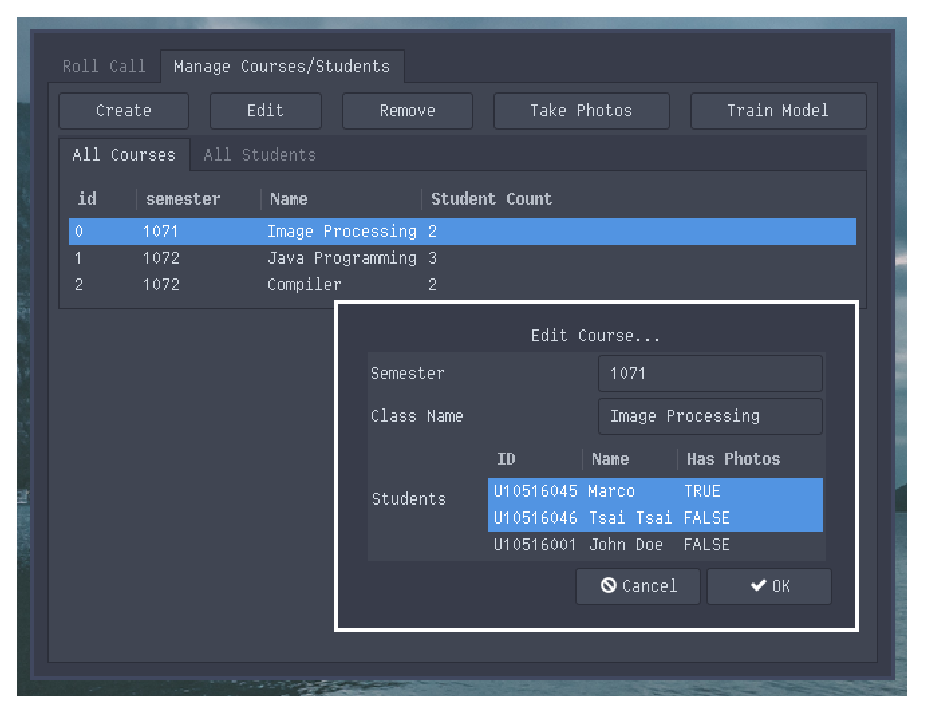
\includegraphics[width=\linewidth]{figures/preview1.eps}
    \caption{Managing courses.}
  \end{subfigure}
  \begin{subfigure}[b]{0.49\linewidth}
    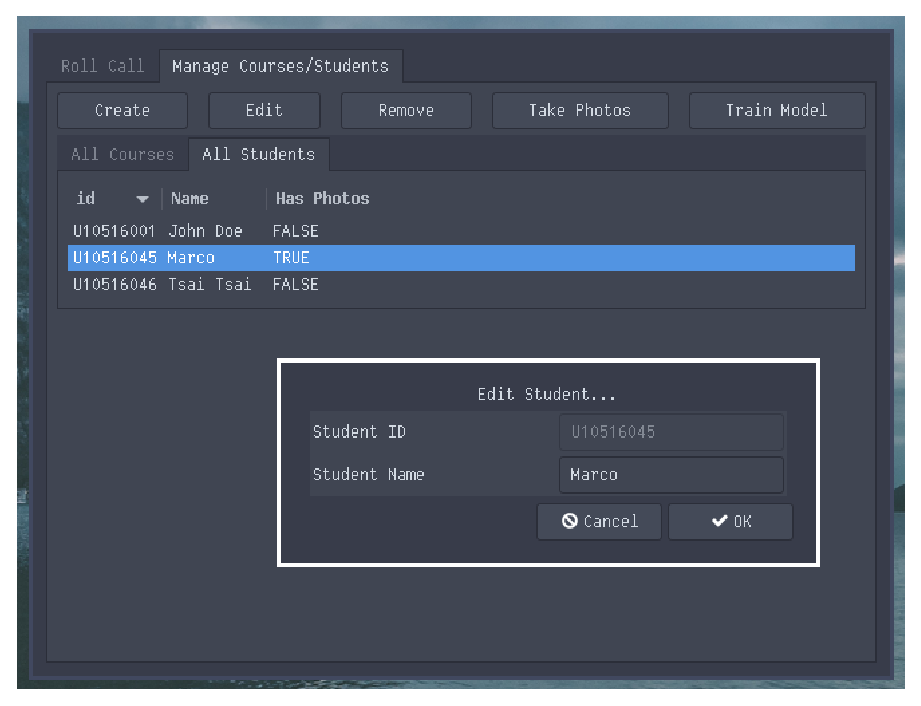
\includegraphics[width=\linewidth]{figures/preview2.eps}
    \caption{Managing students.}
  \end{subfigure}
  \caption{PyRollCall running on a Linux machine with X11\protect\footnotemark \ installed.}
  \label{fig:systemAppearance}
\end{figure}
\vspace{0.5cm}

\footnotetext{X11, also known as X Window System, or simply X, is a windowing system that provides the basic framework for building GUI environments.}

%Another usage of this system is taking the photo of each student one by one as long as
%the size of the class is small enough. If the size of the class is too large, this apparently
%can result in longer waiting time for the students, and hence this approach is impractical.
%Consequently, our main objective is to ensure that the system can accurately recognize all the faces
%in a large image as possible as it can.

The actions available via PyRollCall's GUI are listed as follows:
\vspace{0.5cm}

\setstretch{0.8}
\begin{itemize}
  \item Maintain the data of the course and students they teach.
  \item Take photos of students with a camera and compute the facial embeddings.
  \item Perform roll calls.
  \item Export the results of roll calls to files.
\end{itemize}
\setstretch{\myContentLineSpacing}


\vspace{0.5cm}
Now that we have understood the prerequisites of the facial recognition features in PyRollCall,
it is time that we get to the installation details of this system. PyRollCall is able to run on Windows,
macOS and unix-like systems as long as the system supports Python 3 and GUI applications.
Furthermore, PyRollCall is open-sourced and managed with \emph{git}\footnote{git is a distributed
  version control system used for tracking file content changes in source code during software development},
and all of its external dependencies are already packaged in the project via Python's {virtualenv}\footnote{\
  virtualenv is a tool to created isolated Python environments by maintaining a set of libraries that a specific application depends on.},
thus the users do not have to worry about what and which versions of libraries they need to install. To checkout and run the project:

%Windows and macOS should natively support GUI applications. However, if you are running Linux,
%some distributions such as CentOS, Arch and Gentoo might not, by default, support
%GUI applications. In this case, you'll have to manually install X11 packages on your system.


\begin{lstlisting}[numbers=none,xleftmargin=0em,caption={Shell commands to checkout and run PyRollCall}]
$ git clone https://github.com/aesophor/pyrollcall.git
$ cd pyrollcall
$ source venv/bin/activate
$ ./pyrollcall.py 
\end{lstlisting}

The entry point to the system is \emph{pyrollcall.py}, a script located under the project's root directory.
Before running it, source the shell script \emph{venv/bin/activate} to activate the project's virtual environment.
